\documentclass[12pt]{article}

\usepackage{graphics}
\usepackage{html}
\usepackage{amssymb}
\usepackage{hyperref}

\renewcommand{\familydefault}{\sfdefault}

\setlength{\textwidth} {6.5 true in}
\setlength{\textheight}{9 true in}
\setlength{\hoffset}   {-0.50 true in}
\setlength{\voffset}   {-0.75 true in}

\begin{document}

\section*{Review of Complex Numbers}

\subsection*{Cartesian Form and the Complex Plane}
\begin{itemize}
\item Complex numbers and functions contain the number
  $i = \sqrt{-1}$.

\item Any complex number or function $z$ can be written in
  \textbf{Cartesian form},
  \begin{equation}
    \label{eq:z}
    z = a + i b
  \end{equation}
  where $a$ is the \textbf{real part} of $z$ and $b$ is the
  \textbf{imaginary part} of $z$, often denoted $a = Re\{z\}$ and
  $b = Im\{z\}$, respectively. Note that $a$ and $b$ are both real numbers.

\item The form of Eq.~\ref{eq:z} is called Cartesian, because if we
  think of $z$ as a two dimensional vector and $Re\{z\}$ and $Im\{z\}$
  as its components, we can represent $z$ as a point on the
  \textbf{complex plane}.
  \begin{center}
    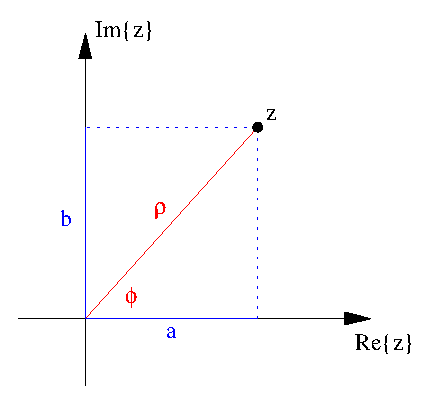
\includegraphics{complex.eps}
  \end{center}

\end{itemize}

\subsection*{Polar Form}
\begin{itemize}
\item As with a two dimensional vector, a complex number can be
  written in a second form, as a magnitude $\rho$ and angle $\phi$,
  \begin{eqnarray}
    \nonumber
    \rho &=& \sqrt{a^2 + b^2}\\
    \tan \phi &=& \frac{b}{a} ~~(+ \pi~\mathrm{if}~a<0) \\\nonumber
    a &=& \rho \cos \phi\\
    b &=& \rho \sin \phi.
  \end{eqnarray}
  where $\phi$ is called the \textbf{complex phase} of $z$.

\end{itemize}

\subsection*{Exponential Form}
\begin{itemize}
\item Euler's formula relates a complex number on the unit circle
  expressed in terms of trigonometric functions to the complex
  exponential function.
  \begin{equation}
    \label{eq:Euler}
    e^{\pm i\phi} = \cos \phi \pm i \sin \phi.
  \end{equation}
  This can be shown by comparing the Taylor series expansions of
  $e^{i\phi}$, $\cos \phi$, and $\sin \phi$. It follows that a complex
  number $z$ can be written in a third form,
  \begin{equation}
    \label{eq:zExp}
    z = \rho e^{i\phi}.
  \end{equation}

  \begin{center}
    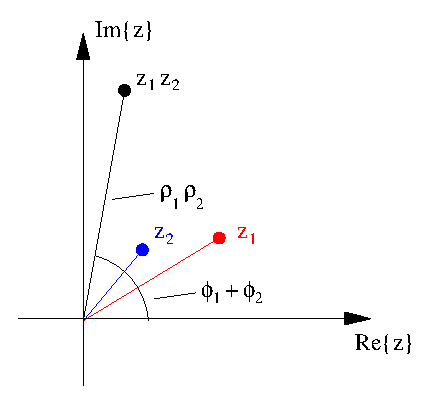
\includegraphics{complexMult.eps}
  \end{center}

\item Eq.~\ref{eq:zExp} provides a useful way of looking at
  multiplication of complex numbers. The product $z_1 z_2$ is 
  obtained by multiplying magnitudes and adding complex phases,
  \begin{equation}
    z_1 z_2 = \rho_1 \rho_2 e^{i(\phi_1 + \phi_2)}.
  \end{equation}

\item Raising complex numbers to powers is also simplified by
  Eq.~\ref{eq:zExp}, 
  \begin{equation}
    \label{eq:zPow}
    (z)^p = \rho^p e^{i p \phi}.
  \end{equation}
  For example, we can evaluate $(i+1)^4$, noting that 
  \[
  1+i = \sqrt{2} \, e^{i\frac{\pi}{4}}
  \]
  and using Eq.~\ref{eq:zPow}, we find
  \begin{eqnarray}
    \nonumber
    (1+i)^4 &=& (\sqrt{2})^4 \, (e^{i\frac{\pi}{4}})^4 
    = 4 \, e^{i\pi} \\
    &=& -4
  \end{eqnarray}

\end{itemize}

\subsection*{Complex Conjugation and the Complex Square}
\begin{itemize}
\item The \textbf{complex conjugate} of $z = a + ib = \rho e^{i\phi}$
  is 
  \[
  z^* = a - ib = \rho e^{-i \phi}.
  \]
  It is obtained by changing the sign of $i$ wherever it appears in $z$.
  \begin{itemize}
  \item To calculate the magnitude $\rho$ directly from $z$ written in
    any form, we use the \textbf{complex square}, 
    \[
    |z|^2 = z^* z
    \]
    The complex square in terms of $a$ and $b$ is
    \begin{eqnarray}
      \nonumber
      |z|^2 &=& (a + ib)(a - ib) = a^2 + iba - iab - (i^2)b^2 \\
      &=& a^2 + b^2 = \rho^2
    \end{eqnarray}
    and in terms of $\rho$ and $\phi$
    \[
    |z|^2 = \rho e^{-i \phi} \rho e^{i \phi} = \rho^2.
    \]
    Hence,
    \begin{equation}
      \rho = \sqrt{|z|^2}.
    \end{equation}

  \item We can also use complex conjugation to separate the real and
    imaginary parts of $z$.
    \[
    z + z^* = a + ib + a - ib = 2a
    \]
    so
    \begin{equation}
    \label{eq:Re}
    Re\{z\} = \frac{z + z^*}{2}
    \end{equation}
    similarly
    \begin{equation}
      \label{eq:Im}
      Im\{z\} = \frac{z - z^*}{2i}
    \end{equation}
    For example, it follows from Eq.'s~\ref{eq:Re} and \ref{eq:Im} together
    with Eq.~\ref{eq:Euler} that
    \begin{eqnarray}
      \nonumber
      Re\{e^{i\phi}\} & = & \cos \phi = \frac{e^{i\phi} + e^{-i\phi}}{2}\\
      Im\{e^{i\phi}\} & = & \sin \phi = \frac{e^{i\phi} - e^{-i\phi}}{2i}
    \end{eqnarray}
  \end{itemize}

\end{itemize}

\subsection*{Finding Roots}
\begin{itemize}
\item $\sqrt[n]{z}$ has $n$ unique values for integer $n$. For
  example, $\sqrt{4} = +2, -2$. In general, some or all of the $n$ roots
  are complex numbers.

\item The cyclical nature of angles means that 
  \[
  z = \rho e^{i\phi},\,\rho e^{i(\phi + 2\pi)}, \,\rho e^{i(\phi + 4\pi)}, \,\rho e^{i(\phi + 6\pi)}, ...
  \]
  all represent the same number.

\item However, if we take the nth root of these representations of
  $z$, we find that there are $n$ unique results with complex phase
  angles less than $2 \pi$.

\item \textbf{Example 1}
  \begin{itemize}
  \item The first 6 representations of $z=8$ are
    \begin{eqnarray}
      \nonumber
      8 &=& 8, \,8e^{i2\pi}, \,8e^{i4\pi}, \\
      &&\,8e^{i6\pi}, \, 8e^{i8\pi}, \,8e^{i10\pi}.
    \end{eqnarray}
    Taking the 6th root, we obtain
    \begin{eqnarray}
      \nonumber
      \sqrt[6]{8} &=& \sqrt{2}, \,\sqrt{2} e^{i \pi/3}, 
      \,\sqrt{2}  e^{i 2\pi/3}, \\
      &&\,\sqrt{2}  e^{i \pi}, \,\sqrt{2}  e^{i 4\pi/3}, 
      \,\sqrt{2}  e^{i 5\pi/3}
    \end{eqnarray}

    The rest of the roots have complex phase $\geq 2\pi$ and all of them
    are alternate representations of the six roots above. 

  \item Graphically,
    \begin{center}
      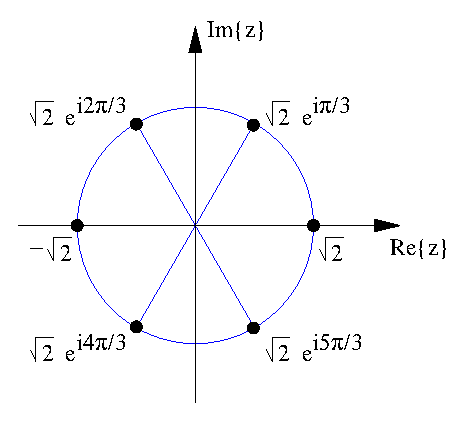
\includegraphics{6roots.eps}
    \end{center}

  \end{itemize}

\item In general, to find the $n$ roots of a number $z = \rho
  e^{i\phi}$, start with $\sqrt[n]{\rho} e^{i\phi/n}$. The remaining
  roots lie, along with the first, on a circle of radius
  $\sqrt[n]{\rho}$ in the complex plane at an equal spacing of $2\pi/n$
  in phase angle.

\end{itemize}

{\footnotesize
  \noindent
  \hrulefill
  
  \noindent
  This work is licensed under the Creative Commons
  Attribution-ShareAlike 4.0 International License: 
  \url{http://creativecommons.org/licenses/by-sa/4.0/}.\\

  \noindent
  L.A. Riley (\texttt{lriley@ursinus.edu}), updated \today
}

\end{document}
